\subsection{Giao diện chỉnh sửa nội dung khảo sát}

\begin{figure}[H]
    \centering
    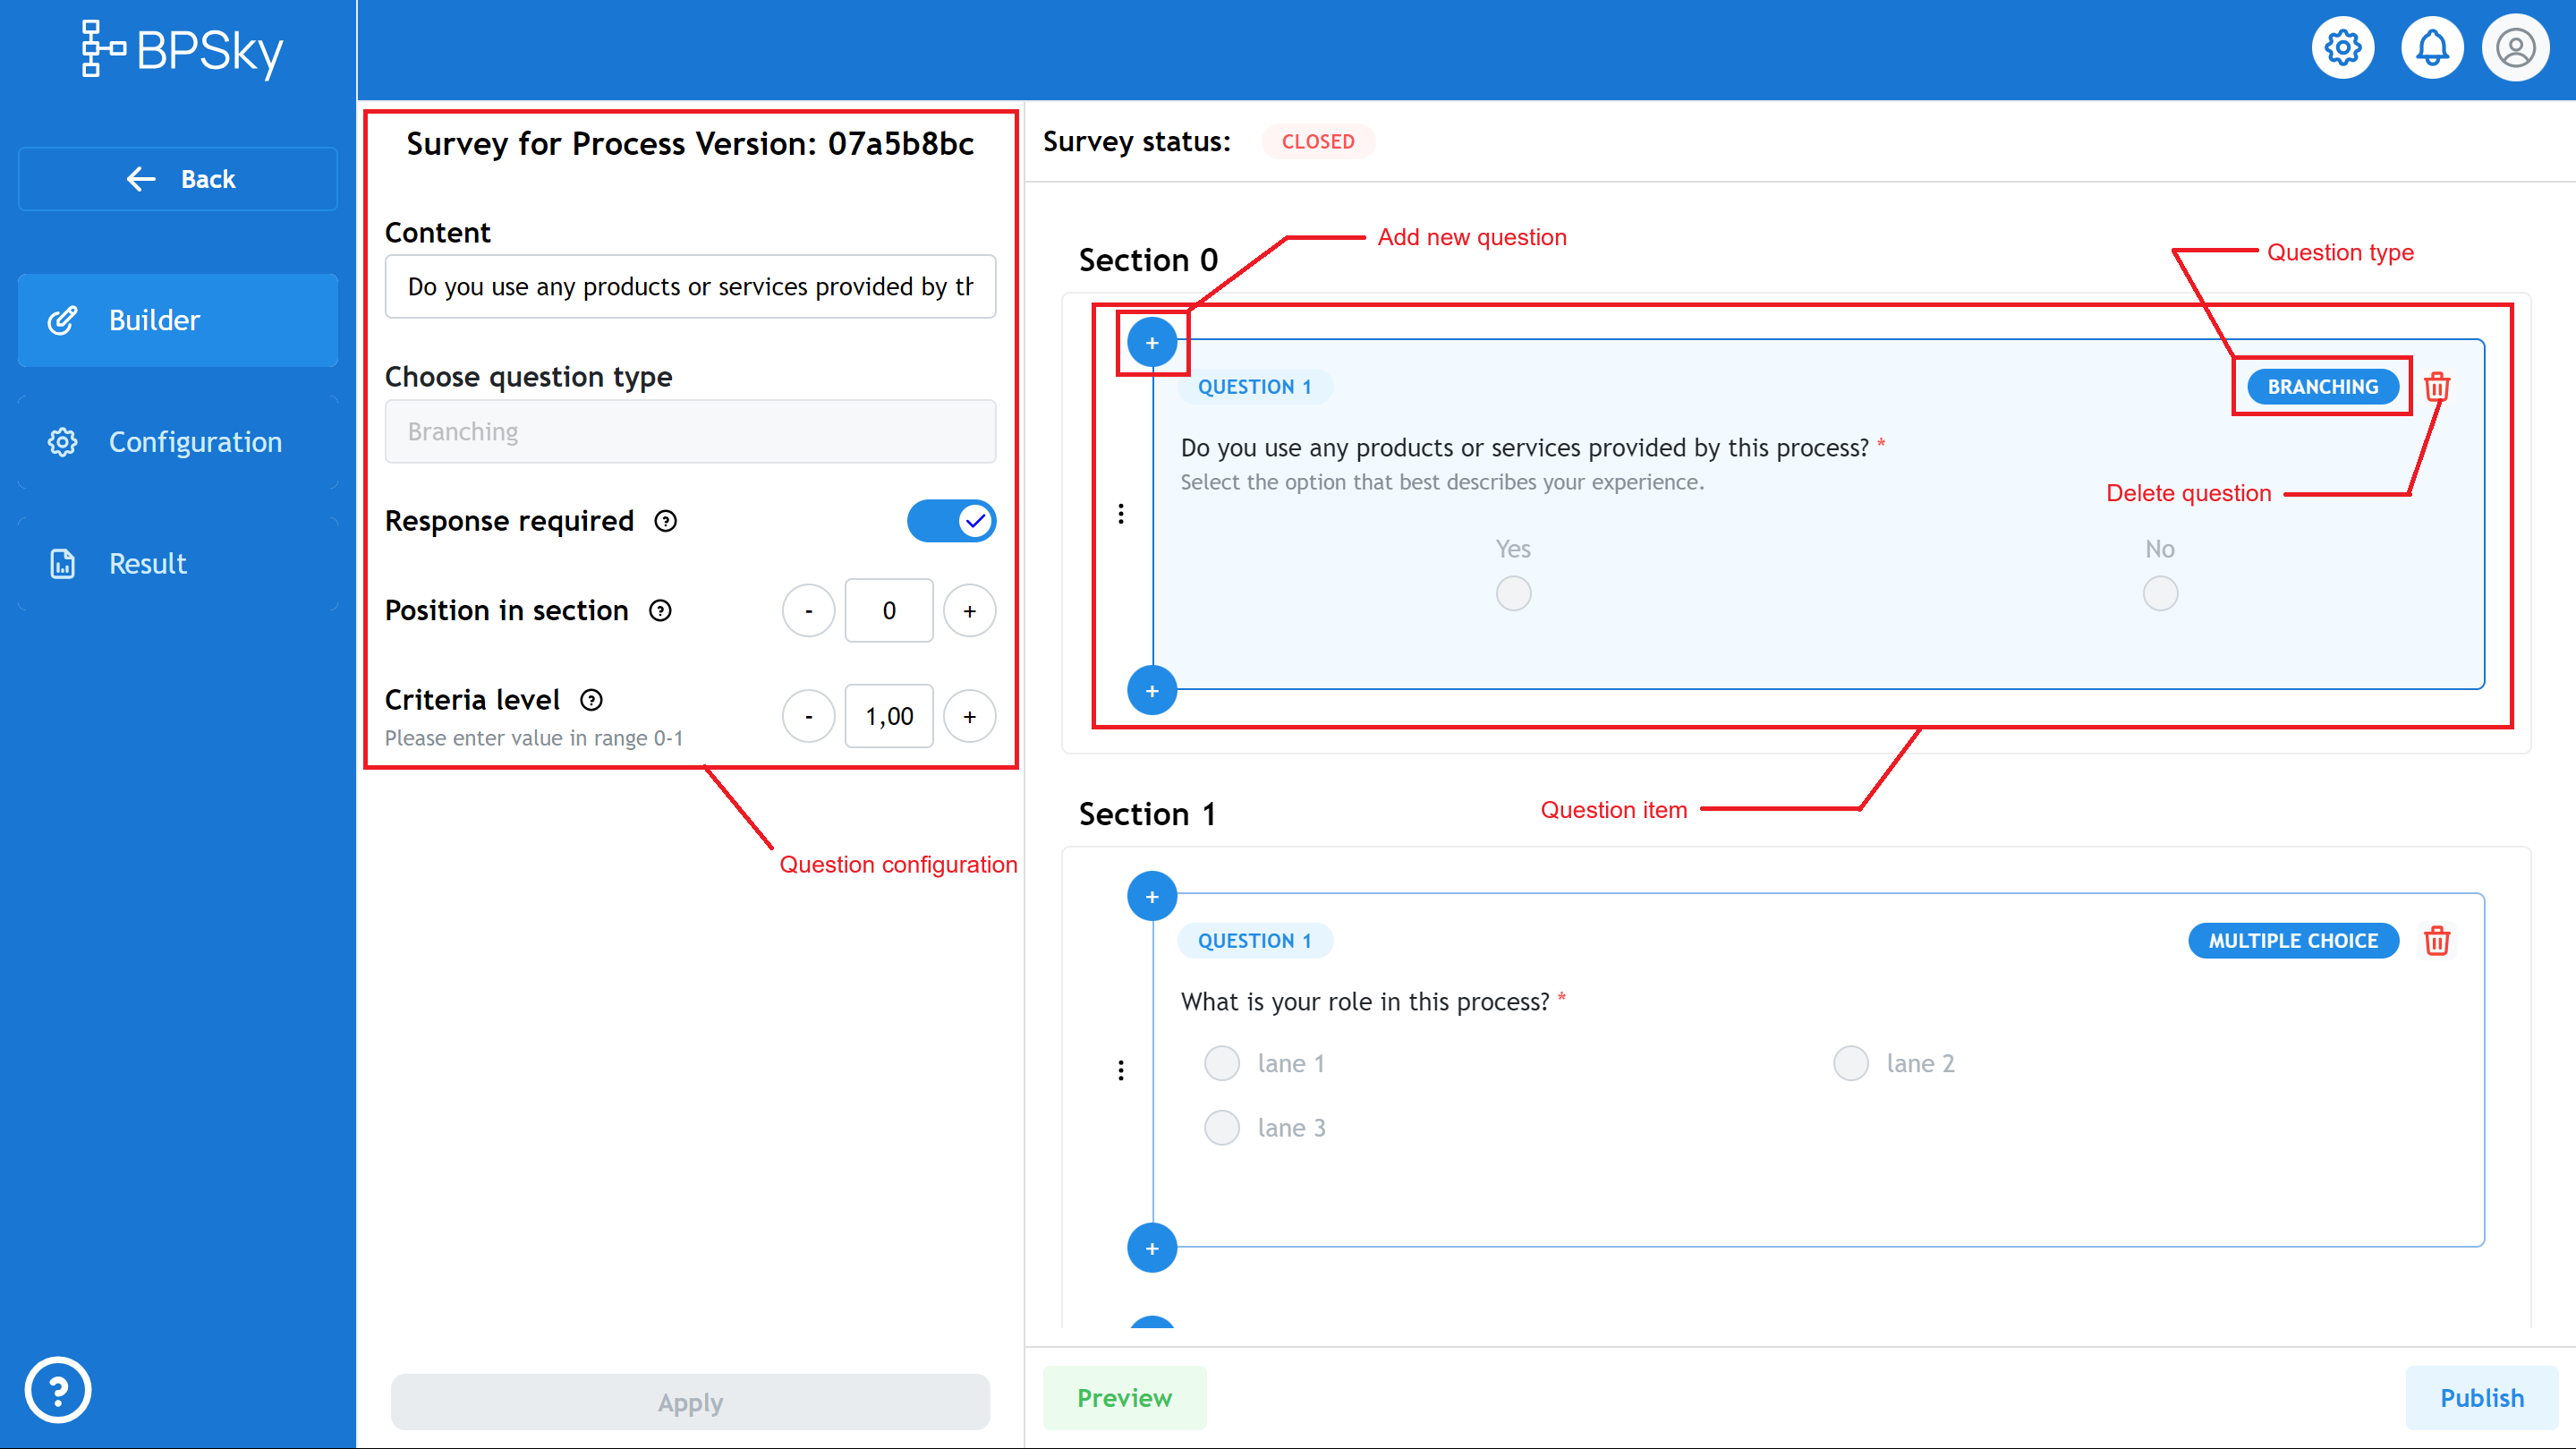
\includegraphics[ width = \linewidth]{Content/Hiện thực hệ thống/documents/Hiện thực giao diện người dùng/images/SurveyBuilder.png}
    \vspace{0.5cm}
    \caption{Giao diện chỉnh sửa nội dung khảo sát}
    \label{fig: Giao diện chỉnh sửa nội dung khảo sát}
\end{figure}

Sau khi chọn biểu tượng khảo sát trên thanh công cụ thì người dùng sẽ được chuyển hướng tới trang giao diện chỉnh sửa nội dung bảng khảo sát. Giao diện chỉnh sửa nội dung khảo sát bao gồm các thành phần sau:

\begin{itemize}
    \item \textbf{Question configuration}: Người dùng có thể chỉnh sửa các thông tin của câu hỏi như tên câu hỏi, loại câu hỏi, câu trả lời (đối với loại câu hỏi multiple question), ...
    \item \textbf{Question item}: Hiển thị nội dung của câu hỏi và thứ tự của câu hỏi trong bảng khảo sát.
    \item \textbf{Question type}: Hiển thị phân loại của câu hỏi, trong phạm vi hệ thống có các loại câu hỏi như NPS, CES, CSAT, CES-IN và CES-IN (dùng thu thập ý kiến của người dùng), Multiple choice và Branching.
    \item \textbf{Delete question}: Dùng để xóa câu hỏi khỏi bảng khảo sát.
\end{itemize}